\documentclass[11pt]{article}
\usepackage{setspace}
\setstretch{1}
\usepackage{amsmath,amssymb, amsthm}
\usepackage{graphicx}
\usepackage{bm}
\usepackage[hang, flushmargin]{footmisc}
\usepackage[colorlinks=true]{hyperref}
\usepackage[nameinlink]{cleveref}
\usepackage{footnotebackref}
\usepackage{url}
\usepackage{listings}
\usepackage[most]{tcolorbox}
\usepackage{inconsolata}
\usepackage[papersize={8.5in,11in}, margin=1in]{geometry}
\usepackage{float}
\usepackage{caption}
\usepackage{esint}
\usepackage{url}
\usepackage{enumitem}
\usepackage{subfig}
\usepackage{wasysym}
\newcommand{\ilc}{\texttt}
\usepackage{etoolbox}
\usepackage{algorithm}
\usepackage{changepage}
% \usepackage{algorithmic}
\usepackage[noend]{algpseudocode}
\usepackage{tikz}
\usetikzlibrary{matrix,positioning,arrows.meta,arrows}
\patchcmd{\thebibliography}{\section*{\refname}}{}{}{}
% \PassOptionsToPackage{hyphens}{url}\usepackage{hyperref}

\providecommand{\myceil}[1]{\left \lceil #1 \right \rceil }
\providecommand{\myfloor}[1]{\left \lfloor #1 \right \rfloor }


\begin{document}



\title{\textbf{CSDS 455: Take Home Midterm}}

\author{Shaochen (Henry) ZHONG, \ilc{sxz517}}
\date{Started on 17:50, submitted before 20:00 10/14/2020 \\ Fall 2020, Dr. Connamacher}
\maketitle



\section*{Problem 1}

Fundation: every complete even graph has a perfect macthing by itself.\footnote{Because every vertex is connected to all other vertices, we may therefore find an arbitrary vertex order of graph $G$ like $\{v_1, v_2, v_3, ..., v_k \}$; by choosing the edges of $v_1 v_2, v_3 v_4, ...$ we will have a perfect matching of $G$.}\newline

We first observe that the number of odd components of $G-X$ must be less than (not equal to) $|X|$. Knowing that vertices in $X$ will connect to every other verticies in $G$, we may group every odd component of $G-X$ with one vertex in $X$ and find a perfect matching out of them (as one odd component should have a matching in itself except one vertex, then by matching this leftover vertex to a vertex in $X$, we have a perfect matching). If the number of odd components of $G-X$ equals to $|X|$, then with the just mentioned grouping operation we will have $|X|$ even components and couple even components in the original $G-X$ set. Then $G$ can't have odd number of vertices, a contradition of the setting.\newline

In the case of the number of odd components of $G-X$ is less than $|X|$. We denote odd components in $G-X$ as $O = \{O_1, O_2, ... \}$ and likewise $E = \{E_1, E_2, ... \}$ for even components. To remove an edge $v$, $v$ must be among $X$, $O$, or $E$.

For $v \in X$, with the just mentioned grouping operation between $X$ and $O$s, we will have couple even complete components (all have a perfect matching by themself) and the leftover of verticies of $X$. This means the leftover of $X$ (after grouping) must be odd in number of verticies, then by removing one $v$ now the leftover of $X$ will be complete and even and therefore has a perfect matching. As every component in $G-v$ now has a perfect matching, $G-v$ has a 1-factor.

For $v \in O$ then we have one odd component $O_i$ become even. By doing the same grouping operation between $X$ and rest of the $O$s. We have $E$s, some even components created by $X$ and $O$s, $O_i - v$, and leftover of $X$ (must be even in verticies as all others are even and $G-v$ is even) -- since all of them are complete and even, an 1-factor can be found.

For $v \in E$, then we have one even component $E_i$ become odd. Since we know $|X| > |O|$, so even with one more odd component we can do the grouping operation between $X$ and all the $O$s. Now we have $E$s, some even components created by $X$ with $O$s or $E_i$, and leftover of $X$ (if any). Since the formor two have even cardinality, the leftover of $X$ must be even. Thus, as all of them are complete and even there will be an 1-factor for $G-v$.\newline

We have showed the statement to be true by justifying all cases.




\section*{Problem 2}

Refer to Dr. Connamacher's MDST algorithm, we have learned that for vertices $x, y$ in a spanning tree $T$ where $d_T(x, y) = diam(T)$, there will always be a midpoint of $x \to y$ path $\chi$ on the edge between $s_1$ and $s_2$. This implies if we try different $\chi$s on different edges and check on their $d_T(x, y) = diam(T)$ respectively, we should be able to locate a tree that has the minimum $diam(T)$.\newline

To generate a SPT rooting from $\chi$ on edge $s_1 s_2$, we may have a $d_T$ with the minimum $\max d_T(s_1, u) + \max d_T(s_2, v) = diam(T)$ for $u, v \in V(G)$\footnote{They also must be leaves of $d_T$ as otherwise we can make the path longer by proceeding to an leave.} as this is the nature of SPT. We learned that there are at most $|V| + 1$ different SPTs can be produced (in a sense of $d_T(s_1, v) \neq d_T'(s_1, v)$ W.L.O.G.) by position $\chi$ differently on $s_1 s_2$. Known there are $|E|$ edges in $G$, we will create $(|V| + 1)|E| = O(VE)$ SPTs.

Use Dijikstra to create SPTs, which has a $O(E \log(V))$ runtime with adjacency list implemented. Also to inspect the $diam(T)$ of each produced SPT, an $O(V + E)$ BFS is required. So to position, create, and inspect all SPTs, we will have a time complexity of $O(V E^2 \log(V) \cdot (V+E))$ in total, a polynomial of number of vertices and edges of $G$.



\section*{Problem 3}


By Menger's theorem we know that for a connected undirecrt graph $G$, the minimum vertex cut for $u, v \in V(G)$ is equal to the maximum number of vertex-disjoint paths from $u$ to $v$. By promoting this theorem to all vertices pairs in $G$, it implies a $k$-connected graph will have $k$ vertex-disjoint pathes between any vertices pair in $G$.

So for a $k+2$ vertex connectivity graph (which is also $k+2$ connected), there will be $k+2$ vertex-disjoint pathes between any vertices pair in $G$. And as the removal of $k$ verticies can at most break $k$ vertex-disjoint pathes, 2 more pathes are left and we may therefore have a cycle between any vertices pair in $G$. So $k+2$ is the minimum vertex connectivity needed for a $k$-resilient graph.

\section*{Problem 4}

By Hall's theorem we know there will be a matching of size $|X|$ by the given condition, but I don't think it will be the case that every edge of $G$ is part of some matching of size $|X|$. Considering the following counter example:

\begin{figure}[H]
    \centering
    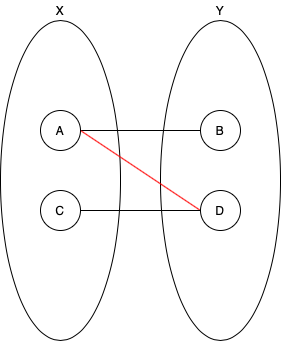
\includegraphics[width=0.25\linewidth]{{fig/fig_p4.png}}
\end{figure}

By selecting $AD$ as a matching edge, we have vertex $A \subseteq X$, we have $|N(A)| = 2$ and $|A| = 1$ therefore $|N(A)| \geq |A|$, so this is a legit graph per requirements. However, edge $AD$ is not in a matching of $|X| = 2$ as it will be the only edge in this matching.\newline

My time is running short but I think this question is provable with the adjustment of $|N(A)| > |A|$ (but not equal). This is because for $A \subseteq X$ we might have an at most $|X|$ matching; and since $|N(A)| > |A|$, when $A = X$ this means we have more edges (than vertices in $A$) available to choose to form a $|X|$ matching. Since the graph is bipartite and $A = X$, all edges in $G$ coorsponding to an $(A, N(A))$ pair. And we can therefore pick any desired edge first and pick the rest $|X| - 1$ edges between the two partition to fullfill a $|X|$ matching.

\section*{Problem 5}

By the $Eular$ therom we have $n - e + f = 2$ for $n, e, f$ representing the number of verticies, edges, and faces of a plane graph $G$. For dual $G^*$ we have $n^* = f$, for isomorphic to $G$ we have $f^* = f$; thus $n^* - e^* + f^* = 2f - e^* = 2$, which implies $e = 2f - 2 = 2n^* - 2$ and we have $e = 2n-2$ again due to isomorphic.


An example will be the following:

\begin{figure}[H]
    \centering
    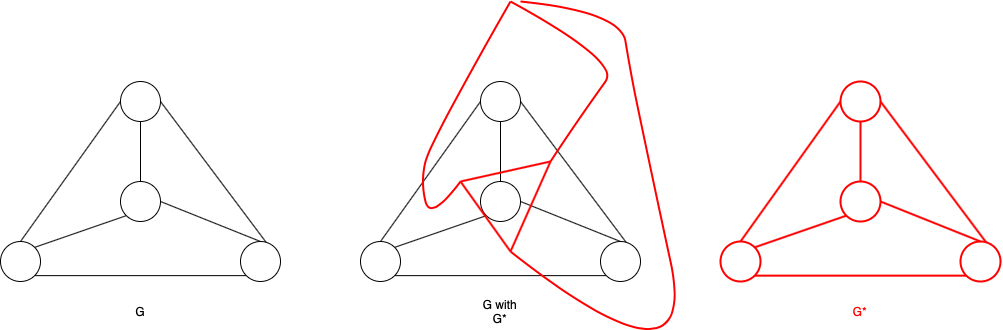
\includegraphics[width=1\linewidth]{{fig/fig_p5.png}}
\end{figure}

Note $G$ has 4 verticies and $2 \cdot 4 - 2 = 6$ edges.\newline


\textit{“I have neither given nor received aid on this examination, and I did not exceed the allowed time.”}\ \ \ \ \ -- HZ.

% \section{References}
%
% \nocite{*}
% \raggedright
% \bibliography{references.bib}
% \bibliographystyle{plain}


\end{document}